	\documentclass[12pt,a4paper,ngerman]{article}
	
	\usepackage[utf8]{inputenc}
	\usepackage[T1]{fontenc}
	\usepackage{babel}
	\usepackage{graphicx} 
	\usepackage{hyperref} 
	\usepackage{pgfplots}
	\usepackage{listings}
	\lstset{numbers=left, numberstyle=\tiny, numbersep=5pt}
	\lstset{language=Java}
	%\usepackage[german]{algorithm2e}
	%\glqq \grqq{}
	\usepackage{tikz}
	\usetikzlibrary{positioning,shadows,arrows}

	\title{Vier Gewinnt}
	\author{}
	
	\begin{document}
	\pagenumbering{gobble}
	\maketitle
	\newpage
	\tableofcontents
	\newpage
	\pagenumbering{arabic}
	\section{Einleitung}
	Das Spiel \glqq Vier Gewinnt\grqq{} erscheint auf den ersten Blick relativ simpel. Nahezu jeder hatte schon Kontakt mit diesem Spiel und hat es sicher einmal oder auch viele Male gespielt. Egal ob auf einem Blatt Papier im Unterricht, mit kleineren oder größeren Spielen aus Plastik, es ist immer ein faszinierendes Spiel für zwei Personen. Es ist nicht so simpel wie z.B. Tic-Tac-Toe, bei dem es bei geübten Spielern immer in einem Unentschieden endet. Bei dem Spiel \glqq Vier Gewinnt\grqq{} geht es viel um das Aufbauen von Fallen, die man dann ausnutzen kann, um zu gewinnen, wenn der Gegenspieler diese ausgelöst hat. Nachdem ich schon einmal ein \glqq Tic-Tac-Toe\grqq{} Spiel mit unbesiegbarem Computergegner programmiert hatte
	%auf der Suche nach einem anspruchsvollerem Spiel; die Wahl fiel auf Vier gewinnt 
	\footnote{\url{https://github.com/boba2fett/TicTacToe}}
	, war mir klar, dass ich bei der Facharbeit dies mit einem  \glqq Vier Gewinnt\grqq{} Spiel umsetzen werde.
	\section{Vier Gewinnt}
	\subsection{Spielidee}
	Die Grundidee des \glqq Vier Gewinnt\grqq{} Spieles ist es vier der eigenen Spielsteine bzw. Symbole in eine Reihe zu bringen.
	Dabei ist es egal, ob dies horizontal, vertikal oder diagonal erreicht wird.
	Es spielen immer zwei Spieler gegeneinander, die abwechselnd einen Spielstein von oben in das Spielfeld einfügen, der dann so lange herunterfällt, bis er auf das Ende des Spielfeldes oder einen anderen Spielstein stößt.
	%einwerfen, herabfallen, setzen
	Sobald zum ersten Mal vier Spielsteine eines Spielers eine Reihe bilden, endet das Spiel und der betreffende Spieler gewinnt.
	Das Spielfeld in der Grundversion ist ein 7x6 Feld. Grundsätzlich sind aber auch größere und kleinere Spielfelder möglich.
	\footnote{Lehmann, Jörg \glqq Vier gewinnt\grqq{} \url{http://www.brettspiele-report.de/vier-gewinnt/} Stand: 01.05.2019}
	\subsection{Implementation}
	Zunächst habe ich ein GitHub-Repository erstellt,um effizient die Versionskontrolle zu nutzen, die den Quelltext auch für andere verfügbar macht.
	Darauf folgend habe ich, wie in der Softwareentwicklung üblich, die Klassendiagramme angelegt,\\
	\textit{Klassendiagramme}\\
	 um diese dann nach Umwandlung in ein Implementationsdiagramm umzusetzen.\\
	\textit{Implementationsdiagramme}\\
	Nach der Umsetzung versuchte ich die Laufzeit etwas zu senken, indem ich eine eigene Klasse erstellte, an deren Objekten die Simulationen durchgeführt wird, um es mehr abzutrennen und die redundante Speicherung der bisherigen Züge zu vermeiden.\\
	\textit{Klassendiagramme VierGame und VierLogik}
	Am Ende des Entwicklungsprozesses habe ich noch eine grafische Oberfläche erstellt, um das Spiel effizienter zu testen. Dabei fiel mir auf, dass die Funktion zu sehen, mit welchen Feldern man gewonnen hat, sehr praktisch ist, da sonst schnell der Überblick und die Lust am Spielen verloren geht.
	\section{Die KI}
	\subsection{Taktik der KI}
	Die Taktik der KI (Künstliche Intelligenz) ist natürlich zu gewinnen oder eine (unmittelbare) Niederlage zu verhindern. Dazu wird ein Minimax-Algorithmus genutzt, um die beste Entscheidung zu treffen. Bei diesem Verfahren durchläuft der Algorithmus einen Suchbaum, der bei der maximalen Suchtiefe jedem Ergebnis einen Wert zuweist oder, wenn schon vorher ein Sieg oder eine Niederlage auftritt, diesen jeweils einen positiven bzw. negativen Wert zuordnet. Bei der Auswertung wird dann immer das Minimum der gegnerischen Züge gewertet und das Maximum der eigenen, so dass jeder Spieler ein \glqq perfektes \grqq{} Spiel spielt. Des Weiteren bevorzugt der Algorithmus einen schnellen Sieg bzw. eine spätere Niederlage.
		\\
	Neben dem Minimax-Algorithmus könnten auch vorberechnete Eröffnungszüge genutzt werden, aber diese unterscheiden sich für jede Spielfeldgröße. Einige Spiele gelten dadurch auch schon als gelöst:
	\begin{figure}[h]
		\centering
		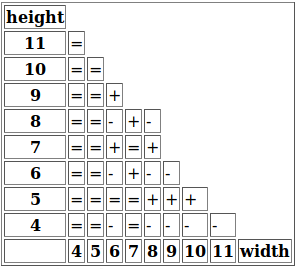
\includegraphics[width=0.5\linewidth, height=0.3\textheight]{w-h-viergew}
		\caption{}
		\label{fig:w-h-viergew}
		\footnote{Tromp, John  \glqq John's Connect Four Playground \grqq{} \url{http://tromp.github.io/c4/c4.html} Stand: 01.05.2019}
	\end{figure}
    \newpage
	Zu Abbildung 1:\\
	+ der 1. Spieler gewinnt\\
	- der 2. Spieler gewinnt\\
	= Unentschieden\\
	
	
	
	\subsection{Schwächen}
	Theoretisch sind der KI mit dem Minimax-Algorithmus nur Grenzen durch die Rechenleistung bzw. die Tiefe der Simulation gesetzt.
	
	\subsection{Implementation}
	Die KI ist in der Klasse AiMiniMax beherbergt. Die dabei wichtigen Methoden sind zum einen die Methoden zum Erzeugen von VierLogik Objekten, an denen die Simulationen durchgeführt werden, und zum anderen die Umsetzung des MiniMax-Algorithmus. Der Aufruf aus VierGame benutzt die Methode aiTurn. In dieser, wird jeder Möglichkeit auf ein Feld zu setzen, ein Wert durch den MiniMax-Algorithmus zugeordnet und danach wird auf das Feld mit dem höchsten evaluierten Wert gesetzt bzw. auf eines der Felder mit dem höchsten evaluierten Wert. Das Herz der KI ist aber der MiniMax-Algorithmus. Der Aufruf erfolgt damit, dass der Zug günstig für den Gegenspieler ist (minimierend für die KI), weil der Zug der KI ja schon für jedes der verfügbaren Felder gemacht wurde, um jedem dieser Felder einen Wert zuzuweisen. Wenn es hier bei einer der durchprobierten Möglichkeiten für den Gegenspieler zu setzen,zu einem Sieg des Gegenspielers kommt, wird ein negativer Wert zugewiesen, der depth entspricht und zurückgegeben wird. Dies sorgt dafür, dass eine spätere Niederlage besser bewertet wird als eine frühe Niederlage.  Bei einem Unentschieden ist der entsprechende Wert 0. Wenn nichts davon eingetreten ist, wird der entsprechende Zug in history gespeichert und der Algorithmus beginnt den nächsten Zug des Spielers zu bewerten. Hier gilt das umgekehrte, da es den Spieler maximiert. Ein früher Sieg bekommt eine sehr positive Bewertung
	%durch Testspieler ist mir aufgefallen, dass die KI sich zu langsam für eine Sieg entscheidet, Im der weiteren Quelltexterstellung/generierung ist aufgefallen, dass die KI denkt, sie hätte nur ein kleineres Feld anstatt des vorhanden 8x8 Spielfeldes.
	 und im nächsten Aufruf ist es wieder minimierend. Wenn die maximale Suchtiefe erreicht ist, wird 0 zurückgegeben und diese Reihenfolge an Zügen wird wie ein Unentschieden behandelt.
	
	\subsubsection{1. Beispiel}
	Nun betrachten wir eine Beispielsituation, wie sie vorkommen könnte und sehen uns genauer an, wie die KI ihre Entscheidung trifft. Diese werden durchgeführt auf einem kleinen Feld von der Größe 4x4 und die KI soll einen Verteidigungszug machen. Damit das Log nicht zu lang wird begrenzen wir die KI auf eine Suchtiefe von 4. Die Ausgaben werden erzeugt durch die Klasse AiMiniMaxPrint.
	Gegeben ist folgende Situation:
\begin{figure}[h]
	\centering
	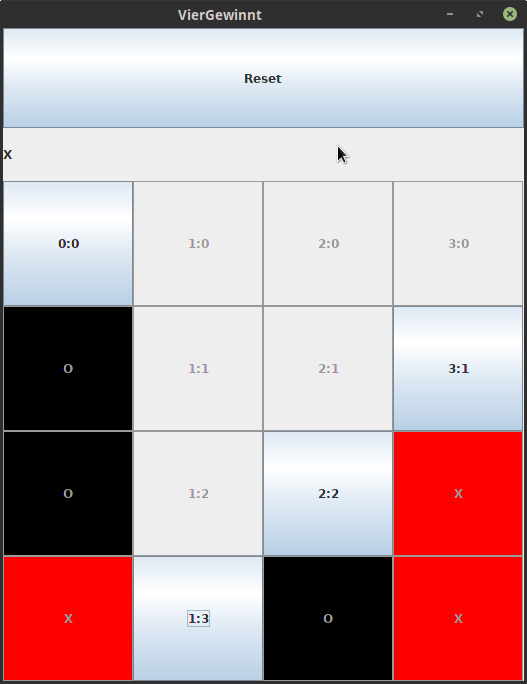
\includegraphics[width=0.4\linewidth, height=0.3\textheight]{maybe/fach0}
	\caption{}
	\label{fig:fach0}
\end{figure}

	Im folgenden setzen wir als Spieler gegen den Computer auf das Feld 3:1, um zu testen, ob er die Bedrohung erkennt.
	
\begin{figure}[h]
	\centering
	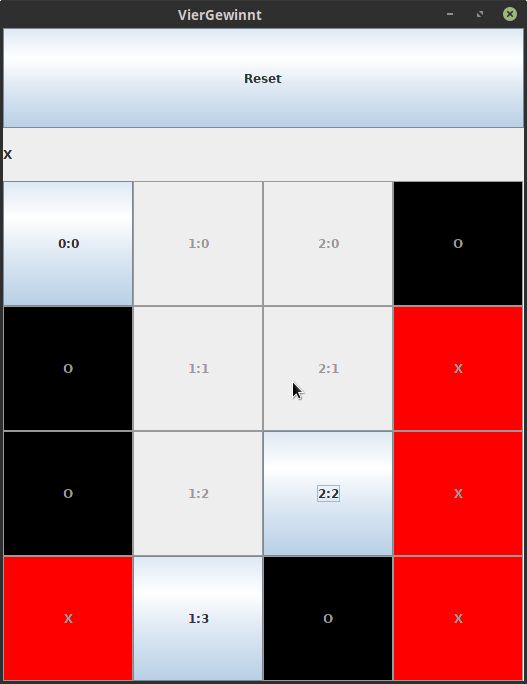
\includegraphics[width=0.4\linewidth, height=0.3\textheight]{maybe/fach1}
	\caption{}
	\label{fig:fach1}
\end{figure}

	Wir erkennen: Das tut er. Aber warum?\\
	Dazu sehen wir uns das generierte Log an:
	\\Anhang\\
	Also die wichtigen Zeilen:\\
	0,3 Defeat\\
	1,3 Defeat\\
	2,3 Defeat\\
	3,return 0\\
	Evaluated Value 0\\
	Consider 3\\
	\\
	Aber was steht hier? Es werden alle Möglichkeiten durchprobiert, bis man in einer maximierenden Ebene auf einen Sieg trifft oder in einer minimierenden auf eine Niederlage. Zeile 1 zeigt, dass wenn der Computer auf 0 setzt, der Spieler mit dem setzen auf 3 Gewinnt. Also eine Niederlage für die KI. Zeile 2 und 3 zeigen das Selbe für den ersten Zug auf 2 oder 3. Zeile 4 hingegen zeigt, dass in den weiteren Stufen bis zur maximalen Suchtiefe keiner durch ein perfektes Spiel gewinnt
	\\
	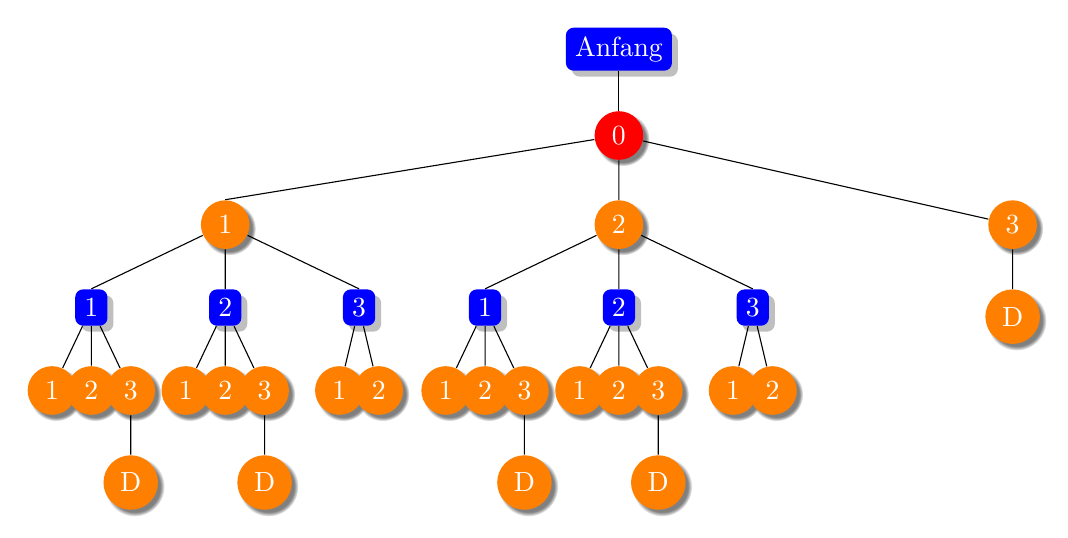
\begin{tikzpicture}[
	max/.style={rectangle, draw=none, rounded corners=1mm, fill=blue, drop shadow,
		text centered, anchor=north, text=white},
	min/.style={circle, draw=none, fill=orange, circular drop shadow,
		text centered, anchor=north, text=white},
	beginn/.style={circle, draw=none, fill=red, circular drop shadow,
		text centered, anchor=north, text=white},
	level distance=0.5cm, growth parent anchor=south
	]
	\node (n) [max,sibling distance=9cm] {Anfang}
child{
	[sibling distance=5cm]
	node (c) [beginn] {0}
	child{
		[sibling distance=1.7cm]
		node (c1) [min] {1}
		child{[sibling distance=0.5cm]
			node (c11) [max] {1}
			child{
				node (c111) [min] {1}
			}
			child{
				node (c112) [min] {2}
			}
			child{
				node (c113) [min] {3}
				child{
					node (c113D) [min] {D}
				}
			}
		}
		child{[sibling distance=0.5cm]
			node (c12) [max] {2}
			child{
				node (c121) [min] {1}
			}
			child{
				node (c122) [min] {2}
			}
			child{
				node (c123) [min] {3}
				child{
					node (c123D) [min] {D}
				}
			}
		}
		child{[sibling distance=0.5cm]
			node (c13) [max] {3}
			child{
				node (c131) [min] {1}
			}
			child{
				node (c132) [min] {2}
			}
		}
	}
	child{
		[sibling distance=1.7cm]
		node (c2) [min] {2}
		child{[sibling distance=0.5cm]
			node (c21) [max] {1}
			child{
				node (c211) [min] {1}
			}
			child{
				node (c212) [min] {2}
			}
			child{
				node (c213) [min] {3}
				child{
					node (c113D) [min] {D}
				}
			}
		}
		child{[sibling distance=0.5cm]
			node (c12) [max] {2}
			child{
				node (c221) [min] {1}
			}
			child{
				node (c222) [min] {2}
			}
			child{
				node (c223) [min] {3}
				child{
					node (c123D) [min] {D}
				}
			}
		}
		child{[sibling distance=0.5cm]
			node (c23) [max] {3}
			child{
				node (c231) [min] {1}
			}
			child{
				node (c232) [min] {2}
			}
		}
	}
	child{
		node (c3) [min] {3}
		child{
			node (c3d) [min] {D}
		}
	}
}
	;
	\end{tikzpicture}
	\\\\
	Hier ist das Baumdiagramm zu 0 als ersten Zug der KI, in dem alle Simulationen angeführt sind, die gemacht werden. Endet ein Pfad im Nichts ist die Maximale Tiefe erreicht, also wie Unentschieden. Steht ein D am Ende eines Pfades ist es eine Niederlage. Blau eingefärbte Knoten sind Maximierende und Orange eingefärbte Minimierende. Fangen wir von links an. Die Maximale Tiefe ist erreicht, also ist der Wert für den Pfad 0-1-1 (Von oben nach unten gelesen) erst mal das Maximum 0. Der nächste Wert von rechts ist wieder 0, also keine Veränderung. Der darauf folgende ist eine Niederlage aber, da es ein maximierender Knoten ist, zählt hier das Maximum, 0. Die beiden Knoten daneben liefern kein anderes Ergebnis und dadurch wird der Wert des Minimierenden Knotens 0-1 auch 0. Für den Knoten 0-2 gilt das Selbe. Der Knoten 0-3 mündet direkt in eine Niederlage und damit einen Negativen Wert (hier -2, da Wert=-Suchtiefe+aktuelle Tiefe). Das Minimum von 0-1, 0-2 und 0-3 ist also -2.\\
	Bei dem Start mit dem Knoten 3 ergibt sich nachher ein Wert von 0, der dann den anderen (0,1,2) bevorzugt wird. Am Ende wird im Log noch niedergeschrieben, dass beim Wert 0 das Feld 3 eine Möglichkeit ist, welches dann auch ausgewählt wird.
	\subsubsection{2.Beispiel}
	Beim zweiten Beispiel wollen wir nun eine Situation herbei führen, bei dem wir in der Zwickmühle sitzen.\\
	\begin{figure}[h]
		\centering
		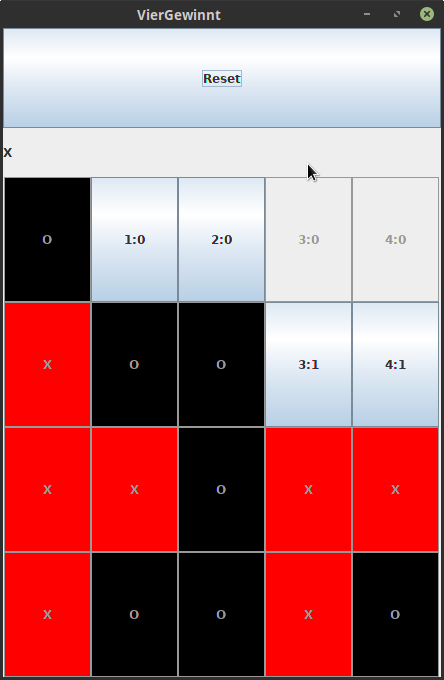
\includegraphics[width=0.4\linewidth, height=0.3\textheight]{maybe/fach2}
		\caption{}
		\label{fig:fach2}
	\end{figure}
	Nun setzen wir als Spieler auf 2:0 um nicht zu verlieren.
	\begin{figure}[h]
		\centering
		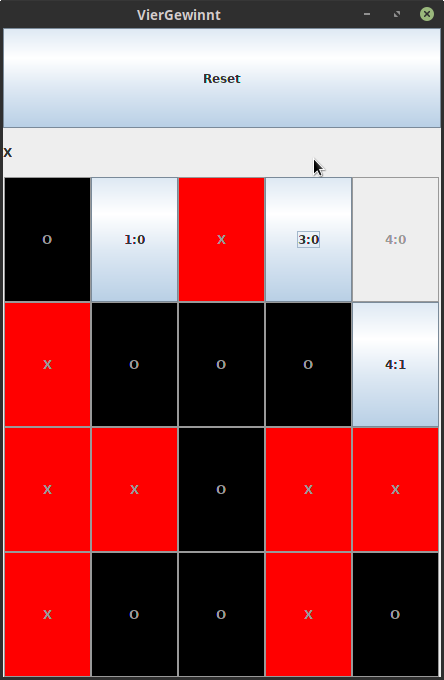
\includegraphics[width=0.4\linewidth, height=0.3\textheight]{maybe/fach3}
		\caption{}
		\label{fig:fach3}
	\end{figure}\\
	Und die KI setzt auf 3:1 und wir haben keine Chance mehr zu Gewinnen. Setzen wir auf 4:1 setzt die KI im nächsten Zug auf 4:0 und gewinnt. Setzten wir hingegen nicht auf 4:1 setzt die KI auf dieses Feld und gewinnt ebenfalls.
	Schauen wir uns nun wieder den Suchbaum an. Er geht hervor aus fach2-3\\
	
	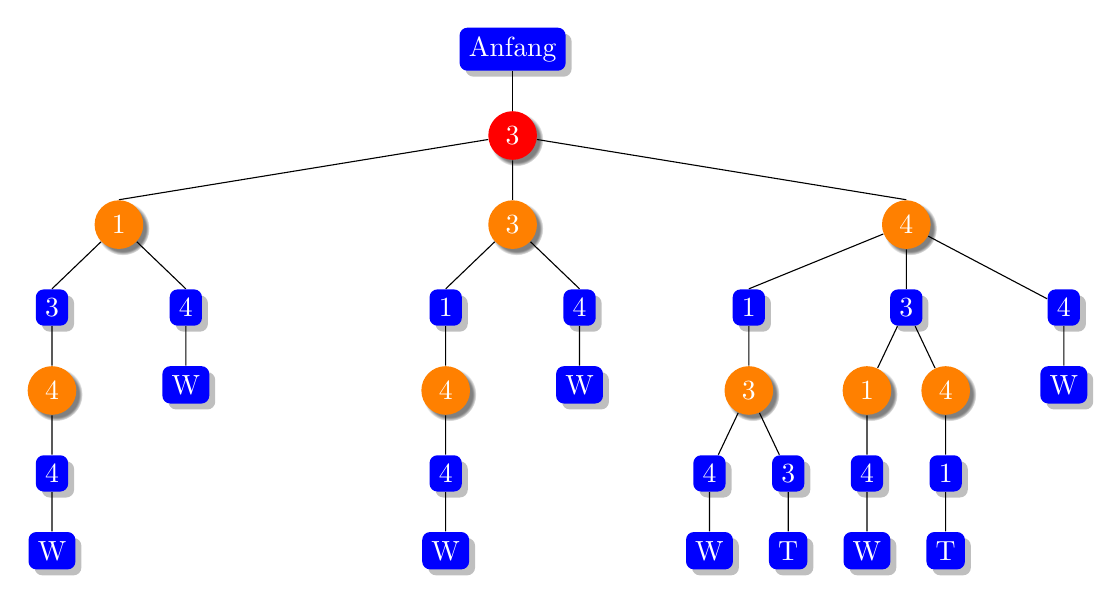
\begin{tikzpicture}[
	max/.style={rectangle, draw=none, rounded corners=1mm, fill=blue, drop shadow,
		text centered, anchor=north, text=white},
	min/.style={circle, draw=none, fill=orange, circular drop shadow,
		text centered, anchor=north, text=white},
	beginn/.style={circle, draw=none, fill=red, circular drop shadow,
		text centered, anchor=north, text=white},
	level distance=0.5cm, growth parent anchor=south
	]
	\node (n) [max,sibling distance=9cm] {Anfang}
	child{
		[sibling distance=5cm]
		node (c) [beginn] {3}
		child{
			[sibling distance=1.7cm]
			node (c1) [min] {1}
			child{[sibling distance=0.5cm]
				node (c13) [max] {3}
				child{
					node (c134) [min] {4}
					child{
						node (c1344) [max] {4}
						child{
							node (c1344W) [max] {W}
						}
					}
				}
			}
			child{[sibling distance=0.5cm]
				node (c14) [max] {4}
				child{
					node (c14W) [max]{W}
				}
			}
		}
		child{
			[sibling distance=1.7cm]
			node (c3) [min] {3}
			child{[sibling distance=0.5cm]
				node (c31) [max] {1}
				child{
					node (c314) [min] {4}
					child{
						node (c3144) [max] {4}
						child{
							node (c3144W) [max] {W}
						}
					}
				}
			}
		child{[sibling distance=0.5cm]
			node (c34) [max] {4}
			child{[sibling distance=0.5cm]
				node (c34W) [max] {W}
			}
		}
		}
		child{[sibling distance=2cm]
			node (c4) [min] {4}
			child{[sibling distance=1cm]
				node (c41) [max] {1}
				child{
					node (c413) [min] {3}
					child{
						node (c4134) [max] {4}
						child{
							node (c4134W) [max] {W}
						}
					}
				child{
					node (c4143) [max] {3}
					child{
						node (c4143T) [max] {T}
					}
				}
				}
			}
		child{[sibling distance=1cm]
			node (c43) [max] {3}
			child{
				node (c431) [min] {1}
				child{
					node (c4314) [max] {4}
					child{
						node (c4314W) [max] {W}
					}
				}
			}
		child{
			node (c434) [min] {4}
			child{
				node (c4341) [max] {1}
				child{
					node (c4341T) [max] {T}
				}
			}
		}
		}
			child{
				node (c44) [max] {4}
				child{
					node (c44W) [max] {W}
				}
			}
		}
	}
	;
	\end{tikzpicture}
	\\
	Oben haben wir nun die Wahl des Feldes 3 die nächste Ebene ist minimierend. Auf der nächsten Ebene ist aber wieder alles Maximierend und es tritt bei jeder Möglichkeit, durch einen schlauen Zug, ein Sieg für die KI ein. Der errechnete Wert ist dabei dann 3 (Suchtiefe - aktuelle Suchtiefe) und dieser Wert wird von keiner der anderen möglichen Felder übertroffen. \\
	Hier das weitere Spiel bis zum Sieg der KI:\\
	\begin{figure}[h]
		\centering
		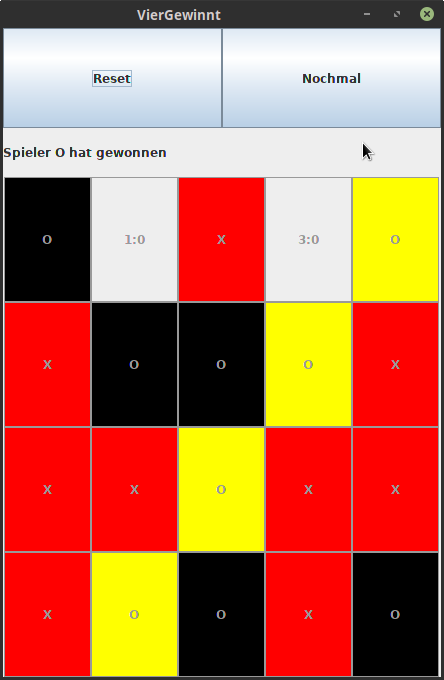
\includegraphics[width=0.4\linewidth, height=0.3\textheight]{maybe/fach4}
		\caption{}
		\label{fig:fach4}
	\end{figure}
	
	\subsection{Effizienzbetrachtung}
	Um mehr Züge zu simulieren, ist erheblich mehr Rechenleistung erforderlich. Die Komplexität steigt nahezu exponentiell, aber je weiter das Spiel fortgeschritten ist und je weniger Möglichkeiten es gibt, desto schneller wird der Algorithmus. Ich habe Simulationen mit verschiedenen Feldgrößen durchgeführt und habe den ersten Zug von der KI berechnen lassen. Dabei habe ich die Zeit gemessen und darauf basierend passende Suchtiefen gewählt, um die Zeit bei weniger als 10 Sekunden zu belassen. Hätte ich die vordefinierten Pfade genommen, wäre deutlich an Rechenzeit gespart worden, jedoch bräuchte man zum Erstellen dieser sehr lange bzw. würde es den Rahmen dieser Facharbeit sprengen. Auch wäre es möglich anstatt der VierLogik Klasse auch einfach nur kopierte Arrays zu verwenden, aber dabei ist es schwer darauf zu achten, dass keines dieser Arrays verändert wird.\\
	Aber nun zur Effizienz bei verschiedenen Feldgrößen. Da die Höhe nicht so ausschlaggebend ist, wird hier nur betrachtet wie sich die Ausführungszeit verändert, wenn die Suchtiefe und die Feldbreite variiert werden. Die KI versucht in jedem Fall, den ersten Zug eines Spieles zu berechnen.\\
	Im Folgenden sind die Graphen der Ausführungszeit im Bezug auf die Suchtiefe dargestellt. Von oben nach unten mit den Feldbreiten 9,7,5. Es fällt deutlich auf, dass bis zu einer Suchtiefe von 5 kaum Unterschiede in der Rechenzeit auftreten. Von da an werden die Unterschiede pro weiterer Suchtiefe immer größer und steigen exponentiell. Der Wert für die Feldbreite 9 und Suchtiefe 9 fehlt, da ich die Messung nach 2 Stunden abgebrochen habe. Die Tests wurden durchgeführt mit der Klasse Testing.\\
	
		\begin{minipage}{\textwidth}
			\centering
		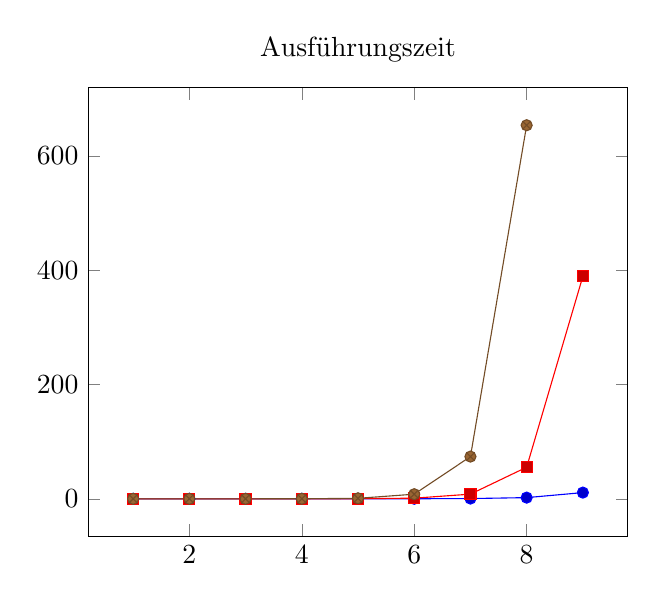
\begin{tikzpicture}
		\begin{axis}[title={Ausführungszeit}]
		\addplot coordinates{%5
			(1,0.002)
			(2,0.001)
			(3,0.007)
			(4,0.027)
			(5,0.022)
			(6,0.122)
			(7,0.451)
			(8,2.104)
			(9,10.888)
		};
		\addplot coordinates{%7
			(1,0.0)
			(2,0.001)
			(3,0.003)
			(4,0.022)
			(5,0.164)
			(6,1.151)
			(7,8.182)
			(8,55.315)
			(9,389.38)
		};
		\addplot coordinates{%9
			(1,0.001)
			(2,0.001)
			(3,0.011)
			(4,0.099)
			(5,0.904)
			(6,8.096)
			(7,73.896)
			(8,653.781)
		};
		\end{axis}
		\end{tikzpicture}
		\end{minipage}
	\section{Künstliche Intelligenz}
	\subsection{Definition}
	Das große Problem beim Begriff künstliche Intelligenz ist, dass es keine allgemeingültige Definition von Intelligenz gibt. Eine Möglichkeit ist es, Intelligenz als Fähigkeit Probleme zu lösen zu sehen. Darunter berücksichtigt wäre auch, dass es verschiedene Arten von Intelligenz gibt. So beschriebt es die \glqq Theorie der multiplen Intelligenzen \grqq{} von Howard Gardner. So habe jeder Mensch eine Mischung aus sieben Intelligenzarten.\footnote{Bulenda, Max \glqq Künstliche Intelligenz: Definition, Erklärung und Beispiele \grqq{}\url{https://simplyki.de/kuenstliche-intelligenz-definition-erklaerung-und-beispiele/} Stand: 10.05.2019} 
	Darauf achtend schauen wir uns den Wikipedia Artikel an, da dort meistens eine gesellschaftlich anerkannte Definition steht.\glqq Künstliche Intelligenz (KI, auch Artifizielle Intelligenz (AI bzw. A. I.), englisch artificial intelligence, AI) ist ein Teilgebiet der Informatik, welches sich mit der Automatisierung intelligenten Verhaltens und dem Maschinellen Lernen befasst. \grqq{} \footnote{Wikimedia Foundation Inc. \glqq Künstliche Intelligenz \grqq{} \url{https://de.wikipedia.org/wiki/K\%C3\%BCnstliche_Intelligenz} Stand: 10.05.2019 }
	Etwas ähnliches  ist auch im Gabler Wirtschaftslexikon zu finden: \glqq Erforschung intelligenten Problemlösungsverhaltens sowie die Erstellung intelligenter Computersysteme. Künstliche Intelligenz (KI) beschäftigt sich mit Methoden, die es einem Computer ermöglichen, solche Aufgaben zu lösen, die, wenn sie vom Menschen gelöst werden, Intelligenz erfordern. \grqq{} \footnote{Prof. Dr. Richard Lackes und Dr. Markus Siepermann \glqq Künstliche Intelligenz (KI) \grqq{} \url{https://wirtschaftslexikon.gabler.de/definition/kuenstliche-intelligenz-ki-40285} Stand: 10.05.2019 }
	Und auch bei Spektrum steht etwas ähnliches: \glqq Die künstliche Intelligenz (Abk. KI, \textit{E} artificial intelligence, Abk. AI) ist ein Teilgebiet der Informatik, welches sich mit der Erforschung von Mechanismen des intelligenten menschlichen Verhaltens befaßt (Intelligenz). Dieses geschieht durch Simulation mit Hilfe künstlicher Artefakte, gewöhnlich mit Computerprogrammen auf einer Rechenmaschine (Computersimulation).\grqq{} \footnote{Wichert, Andreas \glqq Künstliche Intelligenz \grqq{} \url{https://www.spektrum.de/lexikon/neurowissenschaft/kuenstliche-intelligenz/6810} Stand: 10.05.2019 }
	Dementsprechend kann man sagen, dass es sich wohl um die Nachahmung von menschlicher Intelligenz handelt, die durch Computersimulation oder andere Mechanismen erreicht wird.\\
	Damit lässt sich auch für einen Computergegner der Begriff künstliche Intelligenz wählen, da hier durch Computersimulation menschliche Intelligenz nachgeahmt wird.
	\subsection{Machine Learning}
	Ein Teilgebiet der künstlichen Intelligenz ist das Machine Learning ,maschinelles Lernen oder nur ML. Dabei geht es darum aus vorhandenen Daten Muster und Gesetzmäßigkeiten abzuleiten, die dann bei ähnlichen Daten verwendet werden können. Solche lernenden Systeme können über verschiedene wege angelernt werden, aber vor allem die Fortschritte im Bereich Big Data gaben diesem Themenfeld  eine enorme Bedeutung, da nun viele Daten zur Verfügung stehen an denen gelernt werden kann.\footnote{Luber, Stefan \glqq Was ist Machine Learning? \grqq{} \url{https://www.bigdata-insider.de/was-ist-machine-learning-a-592092/} Stand:11.05.2019}
	\subsection{Aktueller Stand}
	Das heutige Leben wäre anders, wenn man auf künstliche Intelligenz verzichten würde. Das mag naheliegend sein bei Google Übersetzer oder anderer Sprachverarbeitung. Aber auch bei Verkehrsmitteln, wie Flugzeugen wird auf KI gesetzt. Man müsse also, um auf KI zu verzichten, mit einer Kutsche fahren. \footnote{Kersting, Pia \glqq Künstliche Intelligenz (KI): Der aktuelle Stand der Technik \grqq{} \url{https://lead-conduct.de/2017/11/21/kuenstliche-intelligenz-ki-der-aktuelle-stand-der-technik/} Stand:11.05.2019}
	es sollte aber im Blick gehalten werden, dass KI unser Leben deutlich vereinfachen kann. So wurde schon 2018 bei der Google I/O demonstriert, wie es aussehen könnte, wenn der Google Assistant einen Termin für seinen Nutzer ausmacht.\footnote{Engelien, Marco \glqq Googles Assistant kann bald euren Friseur anrufen und einen Termin machen \grqq{} \url{https://curved.de/news/bei-anruf-google-der-assistant-macht-bald-termine-fuer-euch-ab-605280} Stand: 11.05.2019}
	\subsection{Ausblick}
	\textit{Filme usw. (Wargames,Terminator,2001,I Robot)}
	
\end{document}

